%%%%%%%%%%%%%%%%%%%%%%%%%%%%%%%%%%%%%%%%%%%%%%%%%%%%%%%%%%%%%%%%%%%
%%% Documento LaTeX 																						%%%
%%%%%%%%%%%%%%%%%%%%%%%%%%%%%%%%%%%%%%%%%%%%%%%%%%%%%%%%%%%%%%%%%%%
% Título:		Capítulo 2
% Autor:  	Ignacio Moreno Doblas
% Fecha:  	2014-02-01, actualizado 2019-11-11
% Versión:	0.5.0
%%%%%%%%%%%%%%%%%%%%%%%%%%%%%%%%%%%%%%%%%%%%%%%%%%%%%%%%%%%%%%%%%%%
% !TEX root = A0.MiTFG.tex

\chapterbegin{Sistema de comunicación}
\label{chp:Utiliz}
\minitoc

\section{Estándar de los sistemas VLC}
%\label{sec:TestSuiteCrec}
La entidad que realiza el estándar es IEEE 802 que realizó el primer estándar oficial de
comunicación por luz visible en 2011 [802.15.7-2011]. Este estándar fue revisado en
2018 y se publicó una segunda versión que es 802.15.7-2018 \textit{IEEE Standard for Local
and metropolitan área networks. Part 15.7: Short-Range Optical Wireless}.

En las comunicaciones ópticas inalámbricas (OWC) los datos se transmiten a través de 
fuentes ópticas, como diodos emisores (LED). Se fusiona la iluminación y las 
comunicaciones de datos en aplicaciones como farolas, letreros, señales de tráfico, 
vehículos etc. Este estándar define el uso de las comunicaciones ópticas inalámbricas.
%https://ieeexplore.ieee.org/stamp/stamp.jsp?tp=&arnumber=8697198
Algunas de las características que se encuentran en el estándar son las siguientes:
\begin{itemize}
    \item Topologías como estrella, P2P (punto a punto) y broadcast (difusión amplia).
    \item Tamaño de direeción (16 o 64 bits).
    \item Acceso aleatorio programado o ranurado con transmisión para evitar colisiones.
    \item Protocolo para transmisiones fiables.
    \item Indicación de la calidad de longitud de onda.
    \item Soporte de atenuación.
    \item Soporte de visibilidad.
    \item Soporte de estabilización de color.
\end{itemize}

%https://ieeexplore.ieee.org/stamp/stamp.jsp?tp=&arnumber=7901496
En esta versión se definen una capa física (PHY) y una subcapa de acceso de control 
al medio (MAC) para comunicaciones ópticas inalámbricas de corto alcance en medios 
ópticamente transparentes que utilizan longitudes de onda de 10000 nm a 190 nm. Es 
capaz de tener velocidad de datos suficiente para admitir tanto servicios de vídeo como 
de audio, así como también considera la movilidad del enlace óptico, su compatibilidad 
con las infraestructuras, los problemas debido al ruido y la interferencia con fuentes 
como la luz natural.

Dependiendo de la aplicación y de la tasa de datos el estándar permite tres tipos de 
capas PHY. PHY I está prevista para aplicaciones exteriores con baja velocidad de 
datos (entre 11.67 kb/s y 267 kb/s). Las capas PHY II y PHY III se proponen para 
aplicaciones de interior con velocidad de datos moderada (entre 1.25 Mb/s y 96 Mb/s).
Esta diferencia se ilustra en la figura \ref{capasPHY}

\begin{figure}[ht]
    \centering
    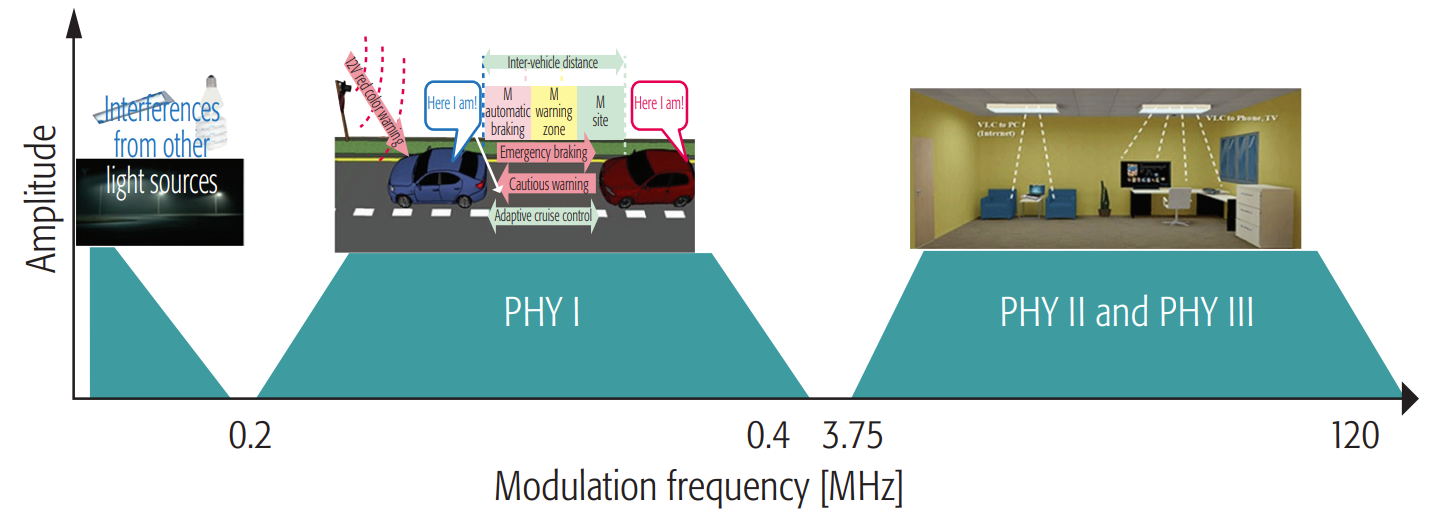
\includegraphics[scale=0.35]{./figuras/capasEstandar.png}
    \caption{\small{División en frecuencia para los tres tipos de capas PHY. Fuente [X].}}
    \label{capasPHY}%
\end{figure}

Además, el estándar especifica tres clases de dispositivos VLC cuyas características 
concretas se muestran en la tabla 1.1. En dicha tabla se puede comprobar como la fuente de 
luz necesaria para la emisión y recepción es débil para móvil, pero debe ser intensa para 
infraestructuras y vehículos. Además, las infraestructuras no incluyen movilidad física 
mientras que tanto móviles como vehículos sí. Una característica muy importante es el 
rango de alcance, este rango es corto para móvil y largo para vehículos mientras que 
para infraestructuras puede ser corto o largo. Por último, se especifica la tasa de datos
(número de bits por unidad de tiempo) que es alta para móvil, baja para los vehículos y 
alta o baja para las infraestructuras.

\begin{table}[ht]
    \centering
    \begin{tabular}{c|
    >{\columncolor[HTML]{CBCEFB}}c |
    >{\columncolor[HTML]{DAE8FC}}c |
    >{\columncolor[HTML]{CBCEFB}}c |}
    \cline{2-4}
                                                                            & \textbf{Infraestructura} & \textbf{Móvil} & \textbf{Vehículo} \\ \hline
    \multicolumn{1}{|c|}{\cellcolor[HTML]{DAE8FC}\textbf{Fuente de luz}}    & Intensa                  & Débil          & Intensa           \\ \hline
    \multicolumn{1}{|c|}{\cellcolor[HTML]{DAE8FC}\textbf{Movilidad física}} & No                       & Sí             & Sí                \\ \hline
    \multicolumn{1}{|c|}{\cellcolor[HTML]{DAE8FC}\textbf{Rango}}            & Corto/Largo              & Corto          & Largo             \\ \hline
    \multicolumn{1}{|c|}{\cellcolor[HTML]{DAE8FC}\textbf{Tasa de datos}}    & Alta/Baja                & Alta           & Baja              \\ \hline
    \end{tabular}
    \caption{\small{Clasificación de dispositivos según el estándar IEEE 802.15.7. Fuente [6]}}
\end{table}

Este estándar proporciona una visión global y común para las comunicaciones ópticas 
inalámbricas de corto alcance. Además, asegura inmunidad a interferencias 
electromagnéticas y a sistemas radiofrecuencia.

\section{Enlace de luz}
Para probar el proyecto y verificar el funcionamiento real del mismo
se parte de un enlace de luz formado por un transmisor y un 
receptor. A continuación, se van a describir brevemente para tener una idea de 
su funcionamiento e importancia ya que han sido 
heredados y no han sido desarrollados en este proyecto. Pero antes la figura 
\ref{enlace}
muestra el enlace completo durante una transmisión a pocos metros en el laboratorio.

\begin{figure}[ht]
    \centering
    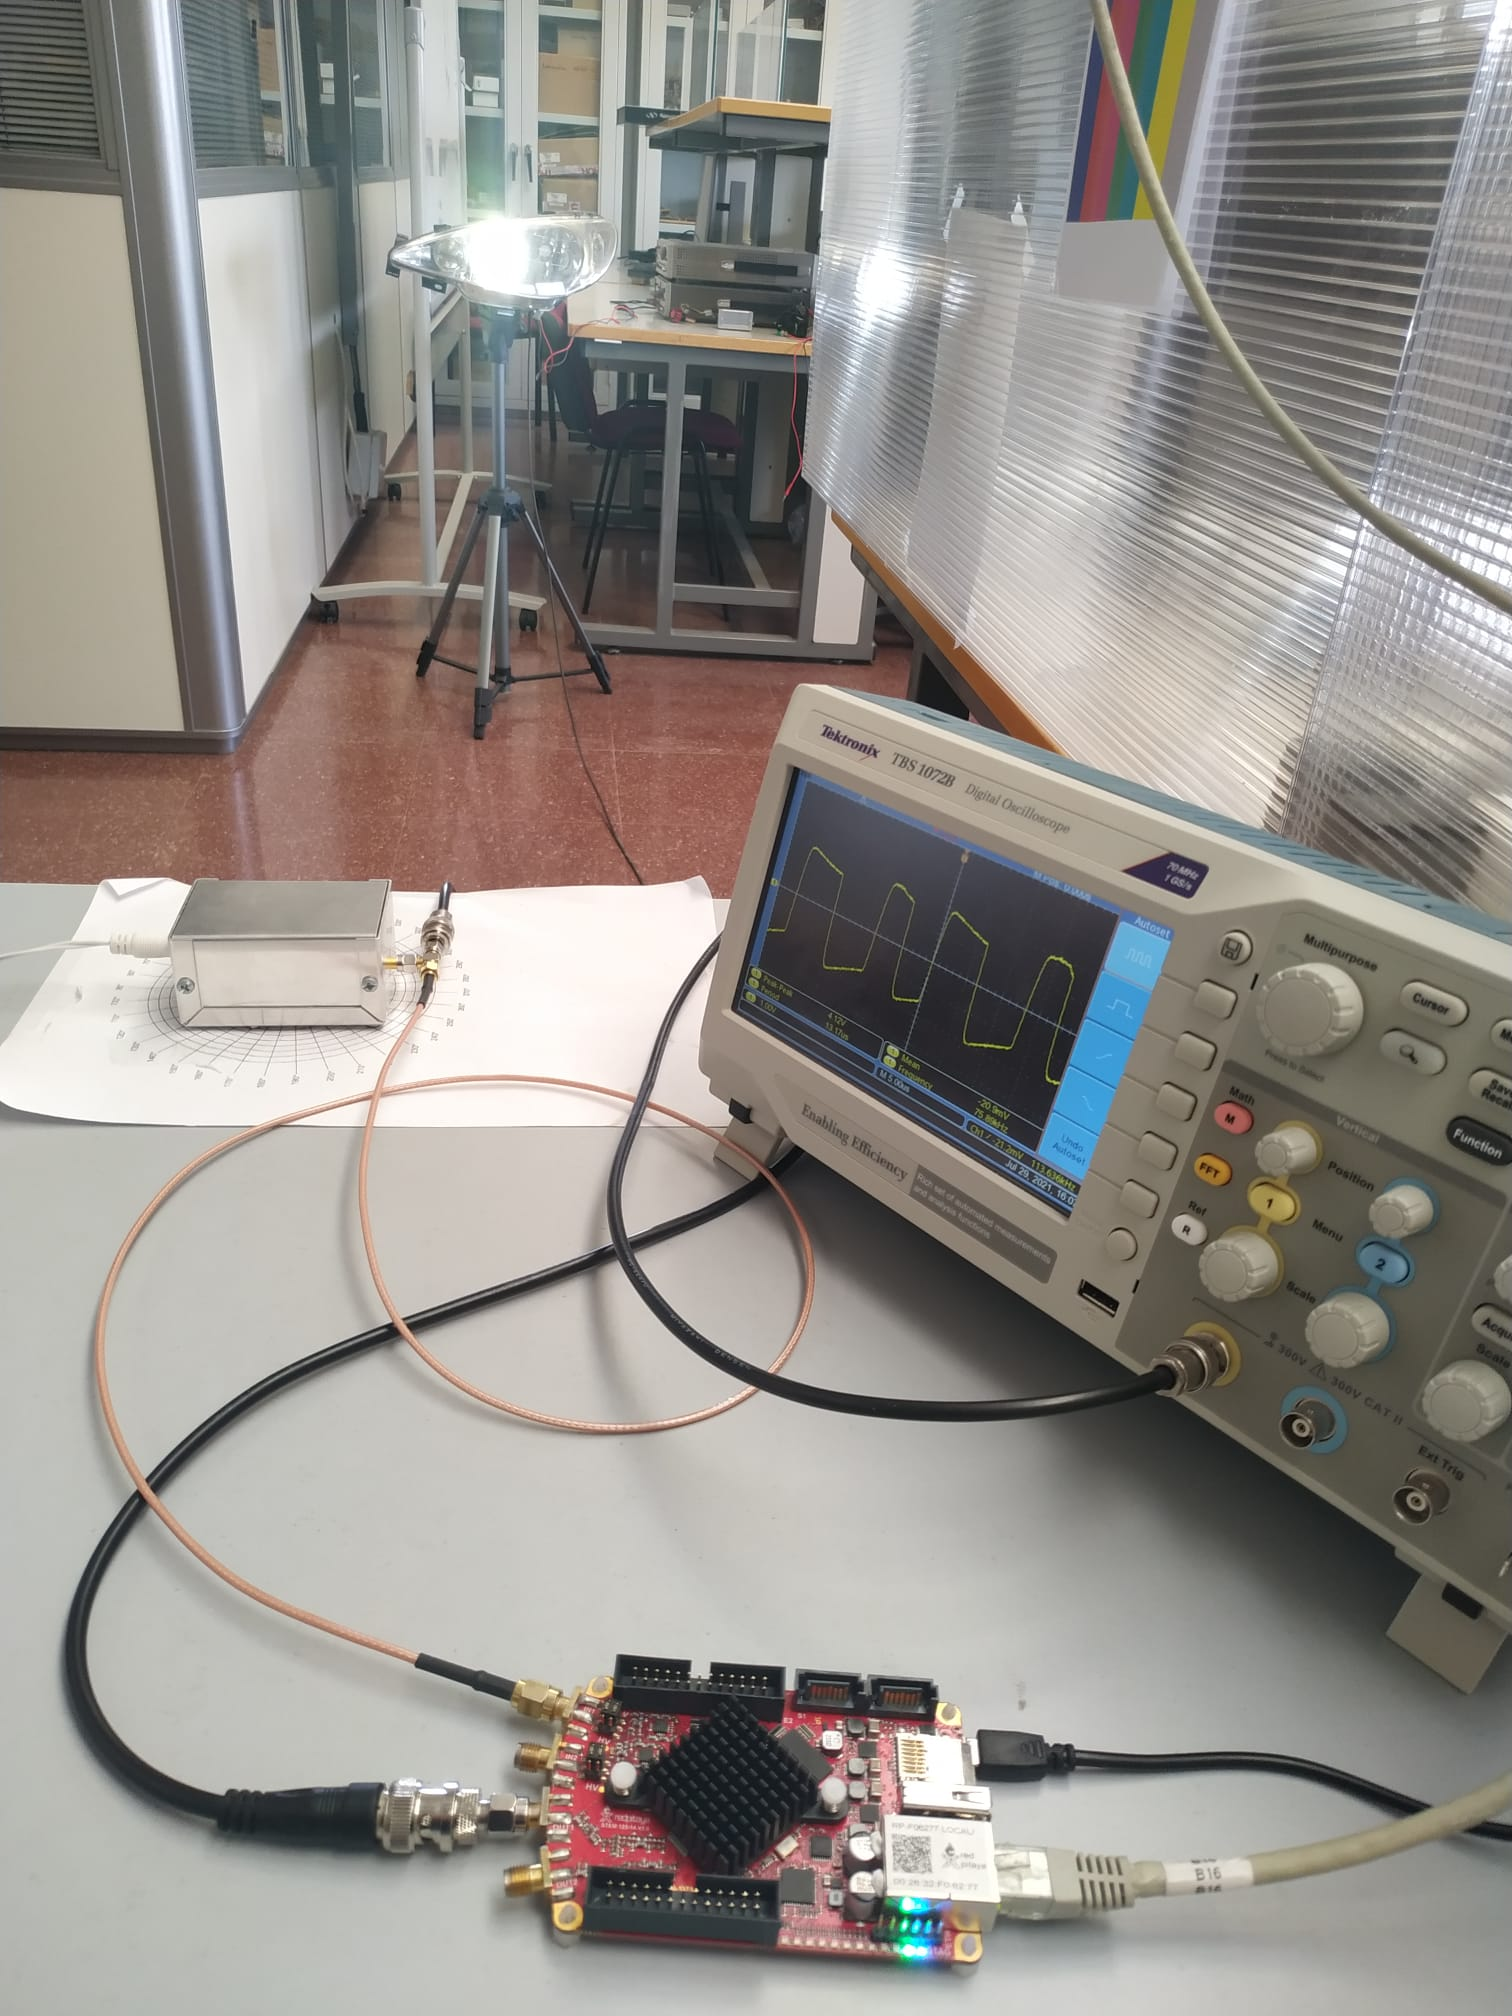
\includegraphics[scale=0.15]{./figuras/Enlace.jpeg}
    \caption{\small{Sistema de transmisión-recepción completo.}}
    \label{enlace}%
\end{figure}

\subsection{Transmisor}
%Hablar un poco del transmisor óptico que tiene Salva y de los voltajes.
El funcionamiento del transmisor se puede desglosar en tres etapas:
\begin{itemize}
    \item Adaptación de nivel: se encarga de convertir los niveles logicos de la señal 
    de entrada ('1' codificado como 1 V y '0' codificado como –1 V) en niveles de tensión 
    utiles para el modulador.
    \item Ajuste de corriente: su función es excitar a los dispositivos
    LED con la corriente reconfigurada.
    \item Habilitación de baja frecuencia: Por debajo de 100 KHz, el nivel de tension alto 
    que se entrega al modulador desciende abruptamente y el ciclo de trabajo de la senal se 
    ve dañado por lo que esta etapa consiste en eliminar dicha restricción.
\end{itemize}

Lo más importante del transmisor es conocer los niveles de amplitud para saber lo que 
tiene que proporcionarle la FPGA. En este caso la amplitud a nivel alto es de 1V y a nivel 
bajo es de 0V. 

En la figura x se muestra una imagen del transmisor óptico.

[FOTO DEL TRANSMISOR DE SALVA]

Este dispositivo ha sido incorporado a un faro de coche para que la simulación de la 
transmisión sea más realista como se ve en la figura x.

[FOTO DEL FARO]

\subsection{Receptor}
%Hablar un poco del receptor óptico que tiene Salva y de los voltajes.
El funcionamiento del receptor se puede desglosar en tres etapas:
\begin{itemize}
    \item Fotodetector: se encarga de transformar la luz pulsada emitida por el transmisor
    en corriente.
    \item Amplificador de transimpedancia: realiza la tarea de convertir la corriente del 
    fotodetector en tensión.
    \item Amplificador no inversor: amplifica la señal para dar más sensibilidad al 
    receptor.
\end{itemize}

Como se comentó en el transmisor lo importante son los niveles de amplitud que, en este 
caso, son de 1V a nivel alto y de -1V a nivel bajo. Este rango es el que tiene la 
FPGA a la entrada por lo que nos proporciona una resolución máxima.

En la figura x se muestra una imagen del receptor óptico.

[FOTO DEL RECEPTOR DE SALVA]

\section{Sistema de partida}
% Hablar sobre el proyecto que nos dejó Andrés tanto de las características
% software como su capacidad de alcance y el enfoque del trabajo de Andrés que era el Desarrollo
% del filtro adaptado y al final tratar de hilarlo con nuestra implementación para mejorar el sistema.
% Comentar el mapeo de la señal para ponerla en el rango [-8192,8191] que nos influye para el hard-decoding y el soft-decoding.
Hay que mencionar que este trabajo coge el testigo de otro trabajo desarrollado con
anterioridad. Dicho trabajo consiste, a grandes rasgos, en el desarrollo del filtro 
adaptado para mejorar la comunción por luz visible. 

El funcionamiento del sistema, de manera general, se divide en dos bloques. Transmisión y 
recepción. 

La transmisión consiste en que un programa en C 
produce una trama que se almacena en la memoria RAM y se pasa a los bloques encargados
de su transmisión como son el serializador, el modulador y finalmente el DAC para 
transformar el dato digital en analógico y el transmisor óptico para transmitir la señal
en forma de pulsos de luz. 

La señal se recibe por el receptor óptico y este la pasa el conversor ADC para volver 
a digitalizar la señal para que pueda ser procesada. Es en este momento, donde actúa el 
filtro adaptado. Su función principal, de una manera resumida, consiste en detectar la 
presencia de una señal conocida o patrón dentro de la señal recibida. La señal a la
salida será la correlación entre la conocida y la recibida. Esto es correspondiente
a realizar la convolución de la señal desconocida con una que usa como referencia.
Por tanto, el objetivo del filtro adaptado es el de maximizar la relación señal a rudi 
(SNR) de una señal conocida para poder recuperarla por completo.

Después de  ser filtrada por el filtro adaptado, la señal se demodula y los datos se 
guardan
en la memoria RAM para que puedan ser leídos el programa en C anteriormente mencionado.

En el siguiente apartado, se van a describir las mejoras que se han decidido
implementar para mejorar sus prestaciones y acercar más el funcionamiento del sistema 
a lo requerido para poder ser implementado en aplicaciones vehículares en las que las 
distancias de transmisión son más largas ya que el sistema anterior no permitía 
transmisiones de larga distancia. 

\section{Mejoras respecto al sistema anterior}
% Hablar sobre cuales son las mejoras que se han implementado y que es lo que se quiere conseguir con estas mejoras.
% Las mejoras (Mayor robustez de paquetes y mayor distancia de transmisión) se han conseguido
% gracias a implementar esquemas de codificación y sistemas de decisión.
Tras analizar el proyecto del que se partía se concluyó que había que desarrollar algún 
subsistema para mejorar el enlace y acercarlo a que pueda ser utilizado en aplicaciones
vehículares de manera eficaz. Una manera de mejorar el 
sistema de comunicación y seguir el camino de investigar los sistemas de comunicación por 
luz visible era desarrollar e implementar varios esquemas de señalización y varios sistemas
de decisión de la señal para analizar sus diferentes comportamientos y cuantificar las 
mejoras. Estas mejoras, principalmente, están centradas en proporcionar mayor robustez al 
sistema para poder interpretar y decodificar la señal de la mejor manera posible cuando
se trabaje en condiciones adversas como pueden ser situaciones en las que la señal se 
mezcle con mucho ruido o simplemente cuando se transmita información a mucha distancia y 
la fuerza de la señal disminuya.

En los siguientes apartados se van a desarrollar tanto su fundamento teórico como su 
implementación en una FPGA tanto de los esquemas de señalización como de los 
sistemas de decisión. Además de realizar las respectivas pruebas para verificar las
mejoras que se producen.

\chapterend{}
